\documentclass[conf]{new-aiaa}

% --- PACKAGES ---
\usepackage{amsmath}
\let\Bbbk\relax % Resolve conflict with newtxmath
\usepackage{amssymb}
\usepackage{booktabs}
\usepackage{graphicx}
\usepackage{url}
\usepackage{algorithm}
\usepackage{algpseudocode}
% \usepackage{cite} % AIAA template uses natbib via new-aiaa class
\usepackage{authblk}
\usepackage{float}
\usepackage{multirow}

% --- GRAPHICS PATH ---
\graphicspath{{figures/}}

% --- TIKZ & GRAPHICS SETUP ---
\usepackage{tikz}
\usetikzlibrary{arrows.meta, positioning, shapes.geometric, calc, backgrounds, fit}

% --- COLOR DEFINITIONS (User Specified) ---
\definecolor{Garnet}{HTML}{73000A}
\definecolor{CSecondaryRed}{HTML}{CC2E40}
\definecolor{CBlue}{HTML}{466A9F}
\definecolor{CDark}{HTML}{1F414D}
\definecolor{COlive}{HTML}{65780B}
\definecolor{CLime}{HTML}{CED318}
\definecolor{CGold}{HTML}{A49137}
\definecolor{CGrayLight}{HTML}{E5E5E5}
\definecolor{CGrayDark}{HTML}{555555}

% --- TIKZ STYLES ---
\tikzset{
    flatblock/.style={
        rectangle,
        draw=black,
        fill=white,
        text width=2.8cm,
        minimum height=1.2cm,
        align=center,
        font=\footnotesize\sffamily,
        line width=0.8pt
    },
    data/.style={
        rectangle,
        draw=Garnet,
        fill=Garnet!5,
        text width=2.8cm,
        minimum height=1.2cm,
        align=center,
        font=\footnotesize\sffamily,
        line width=0.8pt
    },
    decision/.style={
        diamond,
        aspect=2,
        draw=CBlue,
        fill=CBlue!5,
        text width=2.0cm,
        align=center,
        font=\scriptsize\sffamily,
        line width=0.8pt
    },
    flatarrow/.style={
        ->,
        >={Latex[length=3mm, width=2mm]},
        draw=CDark,
        line width=1.0pt
    },
    labeltext/.style={
        font=\scriptsize\sffamily,
        color=CDark
    }
}

\title{Dual-Camera Active Acquisition for Automated Small-Object Dataset Construction}

\author{Jackie Wang\footnote{Graduate Student, Department of Mechanical Engineering, AIAA Student Member, Member ID: 1924106.}}
\author{J.C. Vaught\footnote{Graduate Student, Department of Mechanical Engineering, AIAA Student Member, Member ID: 1537189.}}
\author{Douglas Cahl\footnote{Professor, Department of Mechanical Engineering.}}
\author{Yi Wang\footnote{Professor, Department of Mechanical Engineering.}}

\affil{Department of Mechanical Engineering, University of South Carolina, Columbia, SC, 29208}

\begin{document}

\maketitle

\begin{abstract}
Deep learning performance on small objects is frequently bottlenecked by the quality and quantity of training data rather than model architecture. We present a dual-camera active acquisition system that automates small-object dataset generation by pairing a fixed wide-angle camera for persistent detection with a Pan-Tilt-Zoom (PTZ) camera for optical verification. The system runs concurrent YOLO detector instances on an embedded NVIDIA Jetson Orin AGX platform, achieving 35.9\,FPS on the GPU for wide-area search and 21.5\,FPS on the DLA for PTZ verification. A predictive control framework compensates for mechanical and pipeline latencies to transition from open-loop slewing to closed-loop PID tracking. We demonstrate the system on outdoor drone tracking, where the PTZ autonomously acquires and maintains lock on a small aerial target across a 42-second flight. The active acquisition paradigm replaces digital zoom and super-resolution with true optical zoom, providing ground-truth-quality imagery of targets that occupy fewer than $15 \times 15$ pixels in the wide field.
\end{abstract}

\section{Introduction}
While recent surveys \cite{chen2020survey, nikouei2024smallobj} have demonstrated significant architectural improvements in generic object detection, they have not fully solved a problem that has persisted for decades: small object detection. The core issue remains one of pixel-level information loss, since no amount of digital zoom can recover details that were never sampled. Although some super-resolution algorithms show promise by recovering detail via temporal information, these methods are often computationally intensive and ill-suited for strict real-time inference \cite{mahaur2022superres}.
\par
Even with high-resolution imagery, real-time detection pipelines typically downsample inputs to manageable resolutions (e.g., $640 \times 640$) to satisfy compute constraints. This reduction inherently compresses distant targets into featureless blobs (Fig.~\ref{fig:zoomlevels}) that are difficult to classify without relying on temporal context (as humans do) or additional sensor modalities \cite{rozantsev2017flying}.
\par
\begin{figure*}[htbp]
\centering

\includegraphics[width=1.0\textwidth]{figures/fig_sr_comparison.pdf}
\caption{Comparison of Wide-Angle Crop (Digital Zoom), Super-Resolution, and true Optical Zoom active acquisition.}
\label{fig:zoomlevels}
\end{figure*}

Figure~\ref{fig:zoomlevels} illustrates the challenge in distant aerial surveillance, where a target may occupy fewer than $15 \times 15$ pixels in a wide-angle feed. At this resolution, distractors (i.e.\ birds, cloud edges, specular highlights, or sensor noise) are indistinguishable from the target of interest. Standard digital zooming (cropping) only magnifies these ambiguities \cite{zhang2019zoom}. To achieve robust detection, a dataset must contain examples where these confusing cases are resolved, yet human labelers often cannot distinguish them in raw wide-angle footage.
\par
We address this by replacing the human labeler with a dual-camera system that automates the construction of small-object datasets. A fixed wide-angle camera provides persistent coverage, while a controllable Pan-Tilt-Zoom (PTZ) camera provides resolution on demand. The key technical challenge lies in the handover: the system must move a mechanical lens to capture a moving target based on delayed visual data, compensating for the combined pipeline and mechanical latency.
\par
The contributions of this work are: (i)~a hardware-software architecture that synchronizes wide-angle search with narrow-angle verification on an embedded edge platform; (ii)~a predictive control formulation that compensates for system latency to enable reliable active target acquisition from wide-angle cues; and (iii)~experimental characterization of detector throughput, GPU/DLA parallel inference, and a drone tracking demonstration validating end-to-end system operation.

\section{Related Work}

\subsection{Small Object Detection and Resolution Limits}
The fundamental bottleneck in small object detection is the scarcity of distinguishing features. When a target occupies few pixels (i.e.\ $15 \times 15$ pixels), class-defining details are often lost entirely \cite{nikouei2024smallobj}. Classical solutions involving super-resolution (SR) attempt to reconstruct this lost detail \cite{mahaur2022superres}.

However, reliance on SR for scientific data collection is problematic. First, SR is fundamentally generative; it estimates high-frequency details based on learned priors, creating a risk of hallucination where the model reinforces its own biases \cite{zhang2019zoom}. Second, high-fidelity generative models required for scientific validity often require $>300$\,ms per frame on edge accelerators \cite{nvidia_jetson_benchmarks}, whereas lightweight models sacrifice reconstruction quality. Our system achieves mechanical slew-and-settle in a comparable time window while obtaining true optical ground truth rather than hallucinated details.

\subsection{Active Acquisition vs.\ Continuous Tracking}
Most PTZ tracking literature focuses on the control problem of keeping a target centered in the frame \cite{ptz_reproducible, ptz_eval}. This requires mitigating total system latency (video encoding + network + mechanical response), which for IP-based systems frequently ranges from 200--500\,ms \cite{ptz_latency_optics}. Our work addresses active acquisition, or ``slew-to-classification.'' Unlike continuous tracking, where the objective is persistence, our objective is information gain via discrete spot-checks.

Existing active perception systems like VIGIA-E \cite{vigia_ptz} typically optimize for broad area coverage or anomaly detection. Our system instead functions as a sparse query mechanism: it identifies specific low-confidence candidates in the wide field and commits the PTZ resource to verifying them individually.

\subsection{Sensor-Driven Labeling}
Reducing manual annotation is a central goal of both semi-supervised learning and active learning. Pseudo-labeling methods such as ASTOD \cite{self_training} attempt to retrain models using high-confidence predictions, but this approach often fails in the small-object regime where the detector is consistently uncertain \cite{self_training_enh}. Active learning strategies like PPAL \cite{active_learning_ppod} identify informative samples but still require a human loop \cite{active_learning_survey}.

Our active acquisition creates a fully automated hybrid: the selection logic of active learning (targeting less confident samples) is paired with PTZ verification instead of a human annotator. While the target is ambiguous at $15 \times 15$ pixels, the zoomed view restores it to a regime ($>100 \times 100$ pixels) where off-the-shelf detectors achieve near-perfect accuracy \cite{yolo_flying}. By physically bridging the gap between the surveillance view and the high-resolution training distribution, we convert a difficult small-object inference problem into a trivial classification task.

\section{System Overview and Formulation}
\subsection{Hardware and Software Roles}
The system consists of two FLIR M300C cameras mounted on a shared three-foot stand with a fixed relative pose (Fig.~\ref{fig:hardware}): (1)~a fixed wide-angle camera providing continuous coverage and running a real-time YOLO-family detector on the primary GPU, and (2)~a PTZ camera whose pan, tilt, and zoom are commanded via an HTTP control interface. Both cameras are powered by a 12.8\,V 50\,Ah LiFePO4 battery, selected because the dual-camera current draw exceeded the capacity of a standard DC power supply unit. The cameras connect to an NVIDIA Jetson Orin AGX (JetPack 4.7, CUDA 12.6) via a PCIe Ethernet network card with IEEE~802.3at PoE detection, confirmed safe for the non-PoE FLIR devices. The baseline separation $b \approx 0.5$\,m produces a parallax angle of $\arctan(0.5/100) \approx 0.29^\circ$ at 100\,m range, which is negligible for the initial open-loop slew command.

The software architecture is organized in three layers (Fig.~\ref{fig:gui}). The first layer (L1) provides a Kivy-based GUI with a streamer thread displaying dual camera feeds and exposing controls for zoom, movement speed, tracking mode, and PID tuning parameters. The second layer (L2) runs six threads: a capture thread, a YOLO processing thread, and a draw thread for each camera. The third layer (L3) implements the tracker process, which operates in two phases: Phase~1 performs target acquisition from the stationary camera, and Phase~2 transitions to active tracking on the PTZ camera via a coordinate mapper, centering controller, zoom controller, PID controller, and HTTP command interface. If the PTZ loses detection during Phase~2, the system falls back to stationary camera tracking; once the PTZ reacquires the target, it resumes PTZ-based control.

\begin{figure*}[htbp]
\centering

\includegraphics[width=1.0\textwidth]{figures/fig_zoom_comparison.pdf}
\caption{Visual progression of an active acquisition sequence. A 15-pixel target in the wide field (1x) is indistinguishable from noise. The system cues the PTZ to an intermediate 5x zoom for acquisition, then a 20x zoom for final detailed verification, revealing the aircraft structure clearly.}
\label{fig:zoom_sequence}
\end{figure*}

\begin{figure}[htbp]
\centering
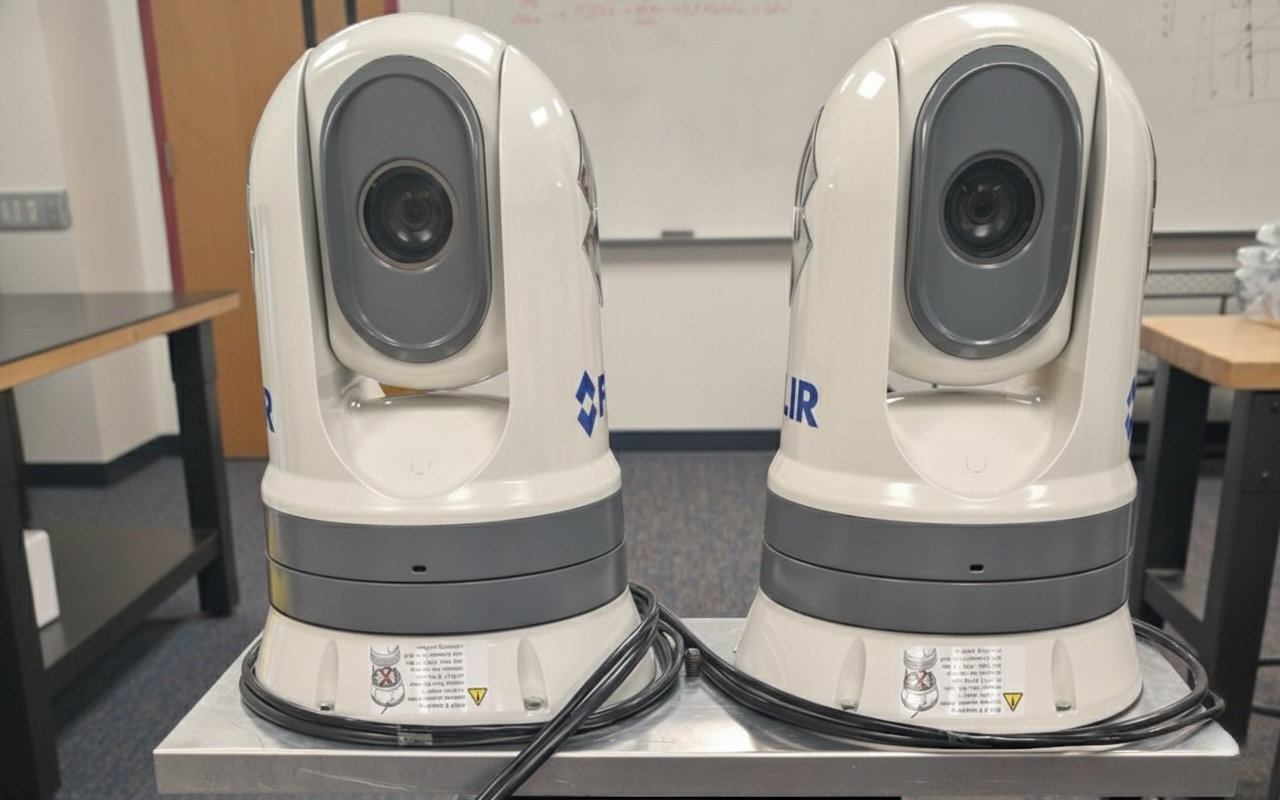
\includegraphics[width=0.75\columnwidth]{figures/fig_hardware_photo.jpeg}
\caption{Physical hardware configuration. Two FLIR M300C cameras are mounted on a shared three-foot stand with $\approx 0.5$\,m baseline separation. The left unit serves as the fixed wide-angle camera; the right unit operates as the PTZ camera.}
\label{fig:hardware}
\end{figure}

\begin{figure}[htbp]
\centering

\includegraphics[width=0.75\columnwidth]{fig_fov_understanding_topdown.pdf}
\caption{Field of view comparison. The wide camera (blue) covers approximately $60^\circ$ horizontally for persistent surveillance, while the PTZ camera (red) provides a narrow, steerable view.}
\label{fig:fov}
\end{figure}

\begin{figure*}[htbp]
\centering
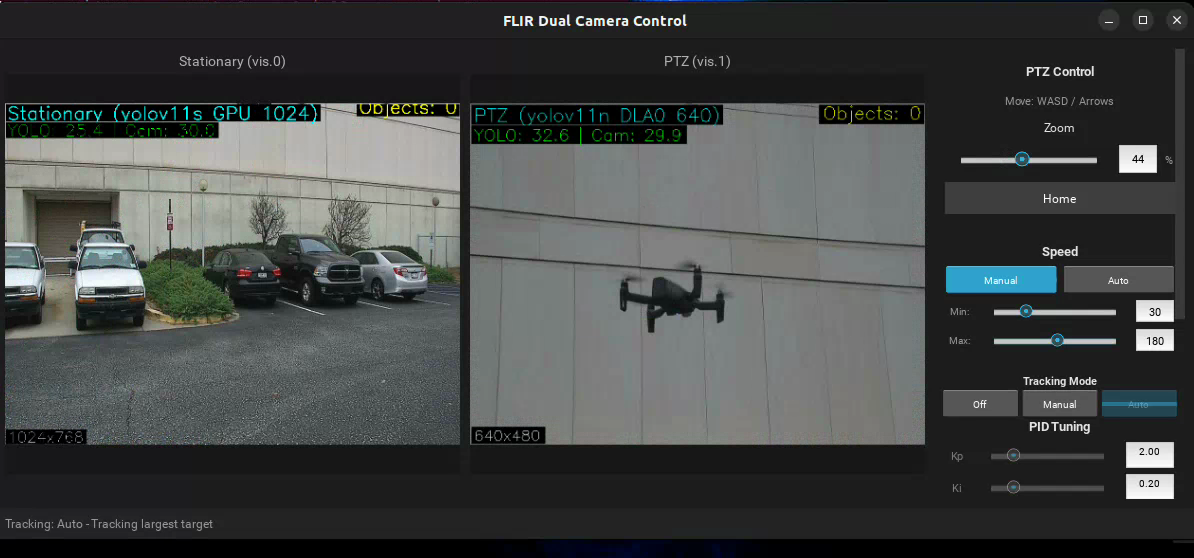
\includegraphics[width=1.0\textwidth]{figures/fig_gui_dual_feed.png}
\caption{Live screenshot of the three-layer software interface during a drone tracking test. The stationary camera (left) runs YOLOv11s on the GPU at $1024\times1024$ resolution for wide-area detection. The PTZ camera (center) runs YOLOv11n on the DLA at $640\times640$, here tracking the drone at optical zoom. The control panel (right) exposes PTZ zoom, movement speed, tracking mode selection, and PID tuning parameters.}
\label{fig:gui}
\end{figure*}

\subsection{Problem Formulation}
We formulate the active acquisition as a greedy utility maximization problem. Let $I^w_{t_{cap}}$ be the wide-angle frame captured at time $t_{cap}$, and let the PTZ state be defined by telemetry $\tau_t = (\theta, \phi, z, \dot{\theta}, \dot{\phi})_t$, explicitly including angular velocity to model inertia. The wide detector produces candidate detections $D_{t_{cap}} = \{(b^w_{i}, s^w_{i}, c_{i})\}_i$.

The system must select an action $a_{t}$ at decision time $t$ that will take effect at a future arrival time $t_{arr} = t + \delta$, where $\delta$ accounts for processing and mechanical slew delays. The objective is to maximize the expected utility of the next captured observation:
\begin{equation}
a^\star = \arg\max_{a \in \mathcal{A}} \mathbb{E}\left[ U(I^p_{t_{arr}}, \tau_{t_{arr}}) \mid D_{t_{cap}}, \tau_{t} \right]
\end{equation}
This optimization is subject to operational constraints: the PTZ must be available (not currently slewing) and the target must be within the reachable field of view. The utility function $U(\cdot)$ prioritizes high-confidence verification, localization precision, and sample diversity.

\section{Calibration and Cross-View Geometry}
\subsection{Camera Model}
Both cameras are modeled with intrinsics $(K_w, K_p)$ and distortion parameters. Let $\Pi(\cdot)$ be perspective projection with distortion, and let $R_{pw}, t_{pw}$ map 3D points from wide-camera coordinates to PTZ-camera coordinates.
\par
For sky targets at long range, parallax between cameras is negligible when the baseline is small relative to range. With a camera baseline of $b = 0.5$\,m and a minimum operating range of $R = 100$\,m, the angular parallax is $\arctan(b/R) = \arctan(0.5/100) \approx 0.29^\circ$. This is well within the PTZ field of view at any zoom level, so a direction-only transfer provides a sufficiently accurate initial seed for the PTZ to acquire the target. Once the PTZ is slewed to this seed location, its onboard detector refines the tracking lock. In this regime, ray directions on the unit sphere are used for cross-view mapping rather than estimated depth.


\subsection{Mapping Wide Detections to PTZ Pan/Tilt Commands}
Let $(u,v)$ be the center of a wide detection box $b^w$ in pixel coordinates. After undistortion, the bearing direction in the wide camera frame is
\begin{equation}
\hat{d}_w = \frac{K_w^{-1}[u \ v \ 1]^\top}{\|K_w^{-1}[u \ v \ 1]^\top\|}.
\end{equation}
Transforming to the PTZ base frame gives $\hat{d}_p = R_{pw}\hat{d}_w$. Using a conventional yaw--pitch parameterization, the commanded pan (yaw) and tilt (pitch) are
\begin{equation}
\theta = \mathrm{atan2}(\hat{d}_{p,y}, \hat{d}_{p,x}), \quad
\phi = \mathrm{atan2}(\hat{d}_{p,z}, \sqrt{\hat{d}_{p,x}^2+\hat{d}_{p,y}^2}).
\end{equation}
Because PTZ motion and video pipelines have latency, $\hat{d}_p$ is preferably computed from a short-horizon prediction of target motion rather than the instantaneous detection center.

\subsection{Zoom Selection by Target Angular Size}
Let $h^w$ be the detected box height in wide pixels. Under small-angle approximation, the apparent angular height is approximately $\alpha \approx h^w / f_w$, where $f_w$ is the wide focal length in pixels. To obtain a desired PTZ pixel height $h^p_{\mathrm{des}}$, select a PTZ focal length $f_p(z)$ such that
\begin{equation}
h^p_{\mathrm{des}} \approx \alpha f_p(z) \approx \frac{h^w}{f_w} f_p(z),
\end{equation}
then choose the zoom $z$ whose calibrated $f_p(z)$ best matches the required value, clipped to PTZ limits. This approach avoids explicit range estimation and is well suited for distant aircraft.


\section{PTZ Triggering, Tracking, and Scheduling}
PTZ tracking is a coupled perception-and-control problem with dynamic imaging conditions and control delays. Prior PTZ tracking evaluations emphasize that camera motion, latency, and re-centering quality dominate performance differences in practice.
\par
We use wide-camera tracklets to provide temporal coherence and to predict target bearing during PTZ motion. A lightweight predictor (e.g., constant angular velocity with $\alpha$--$\beta$ filtering or a Kalman filter) provides a predicted bearing $\hat{d}_w(t+\Delta)$ given command latency $\Delta$, consistent with classical pan/tilt tracking formulations.



\begin{figure}[htbp]
\centering

\includegraphics[width=\columnwidth]{fig_pipeline.pdf}
\caption{Automated label-generation pipeline. Wide-field tracking selects candidates, PTZ verifies optically, and homography maps labels to the wide view.}
\label{fig:pipeline}
\end{figure}

\begin{algorithm}[htbp]
\caption{Real-time wide-to-PTZ acquisition}
\begin{algorithmic}[1]
\State Init $f_{\theta}$ (wide), $\mathcal{T}$ (tracker), $g$ (PTZ), $\mathcal{D}$ (data)
\For{each wide frame $I^w_t$}
\State $D_t \leftarrow f_{\theta}(I^w_t)$; \quad $\mathcal{T}\leftarrow \mathrm{UpdateTracks}(\mathcal{T}, D_t)$
\State Compute $U(o)$ for tracks (conf, size, novelty)
\State Select $o^\star \leftarrow \arg\max U(o)$ s.t. availability
\If{$U(o^\star)>\tau_{\mathrm{trigger}}$}
\State Predict $\hat{d}_w(t+\Delta)$; map to $(\theta,\phi, z)$
\State Command PTZ: $g(\theta,\phi,z)$; get $I^p_{t'}$, $\tau_{t'}$
\State Run PTZ detector: $D^p_{t'} \leftarrow f_{\theta_p}(I^p_{t'})$
\If{Quality OK AND $\max s^p > \tau_{\mathrm{confirm}}$}
\State $b^{w\leftarrow p} \leftarrow \mathrm{Project}(b^p,\tau_{t'})$
\State Commit $(I^w_t, b^{w\leftarrow p}, c)$ to $\mathcal{D}$
\EndIf
\EndIf
\EndFor
\State Periodically retrain $f_{\theta}$ on $\mathcal{D}$
\end{algorithmic}
\end{algorithm}

\subsection{Utility Function for Triggering and Redundancy Control}
The trigger utility balances value and cost. A practical form is a weighted sum of terms:
\begin{equation}
U(o) = \lambda_1\,\mathrm{Unc} + \lambda_2\,\mathrm{SizeGain} + \lambda_3\,\mathrm{Novelty} - \lambda_4\,\mathrm{Cost},
\end{equation}
where $\mathrm{Unc}$ increases when the wide detector is unsure (so PTZ confirmation is valuable), $\mathrm{SizeGain}$ estimates how much the PTZ will increase target pixels, $\mathrm{Novelty}$ reduces redundancy by down-weighting near-duplicates, and $\mathrm{Cost}$ captures PTZ time-on-target, slew distance, and opportunity cost (only one PTZ target at a time). In the current implementation, the system triggers on the largest detected target with confidence above the acquisition threshold ($s > 0.40$), corresponding to a simplified policy where $\lambda_1 = 0$ and the system always acquires available targets.

\section{Automated Dataset Construction}
\subsection{Label Sources and Cross-View Transfer}
The PTZ view is treated as a higher-fidelity label source when it produces a confirmed detection for the target class. The label transfer module maps the PTZ detection back into the wide image coordinate system.
\par
For distant targets, direction-only transfer proceeds by converting the PTZ bounding box corners into bearing rays, rotating those rays into the wide camera frame, and projecting them into the wide image plane. Let $(u^p_k,v^p_k)$ be PTZ box corners; compute PTZ rays $\hat{d}^p_k$ from $K_p^{-1}$, rotate to wide frame $\hat{d}^w_k = R_{wp}\hat{d}^p_k$, then project:
\begin{equation}
[u^w_k, v^w_k, 1]^\top \propto K_w \hat{d}^w_k, \quad k \in \{1,2,3,4\}.
\end{equation}
The transferred wide box is the tight axis-aligned rectangle enclosing the projected corners.

\subsection{Quality Gates and Drift Prevention}
Self-training and pseudo-labeling can suffer from confirmation bias if low-quality pseudo-labels are admitted. In this system, the primary drift control mechanism is the physical zoom verification: many ambiguous wide detections become unambiguous at higher resolution. Remaining failure modes are handled by quality gates that reject samples when motion blur is excessive, exposure is saturated (e.g., sun glare), the target is at the frame boundary, or the PTZ detector disagrees with the wide detector class. Each gate is implemented as a deterministic predicate so that dataset inclusion is reproducible and auditable.

\subsection{Dataset Schema}
Each committed example stores the wide frame (or short clip), the transferred label, and acquisition metadata. Table~\ref{tab:schema} defines the record schema.

\begin{table}[htbp]
\centering
\caption{Dataset record schema for each accepted acquisition.}
\label{tab:schema}
\begin{tabular}{@{}ll@{}}
\toprule
Field & Description \\
\midrule
timestamp\_w & Wide-frame timestamp (monotonic) \\
image\_w & Wide image (or video clip key) \\
bbox\_w & Label box in wide coordinates \\
class & Target class (airplane for the test case) \\
score\_w & Wide detector confidence at time $t$ \\
timestamp\_p & PTZ-frame timestamp used for confirmation \\
telemetry\_p & PTZ pan/tilt/zoom, focus, exposure \\
bbox\_p, score\_p & PTZ detector box and confidence \\
quality\_metrics & Blur, saturation, occlusion flags \\
site\_meta & Location, camera orientation, weather \\
\bottomrule
\end{tabular}
\end{table}

\section{Experimental Validation}

\subsection{System Configuration}
The complete system runs on an NVIDIA Jetson Orin AGX with JetPack~4.7 and CUDA~12.6. Table~\ref{tab:sysconfig} summarizes the hardware and software configuration. The stationary wide camera provides a $60^\circ \times 45^\circ$ field of view for persistent surveillance, while the PTZ camera operates at configurable zoom levels of 25\%, 35\%, and 45\% during tracking.

\begin{table}[htbp]
\centering
\caption{System hardware and software configuration.}
\label{tab:sysconfig}
\begin{tabular}{@{}ll@{}}
\toprule
Component & Specification \\
\midrule
Compute platform & NVIDIA Jetson Orin AGX \\
Software stack & JetPack 4.7, CUDA 12.6 \\
Cameras & 2$\times$ FLIR M300C \\
Power & 12.8\,V 50\,Ah LiFePO4 \\
Network & PCIe Ethernet, IEEE 802.3at PoE \\
Camera latency & 0.2--0.6\,ms (network) \\
Wide FOV & $60^\circ$H $\times$ $45^\circ$V \\
Video codec & MJPEG (frame-independent) \\
\bottomrule
\end{tabular}
\end{table}

\subsection{Detector Throughput}
The two detector instances are split across compute units to avoid GPU time-slicing overhead. The stationary camera runs YOLOv11s on the GPU, where larger model capacity aids feature extraction on distant, low-resolution targets. The PTZ camera runs YOLOv11n on the DLA, where zoomed-in targets are easier to classify. This split achieves true parallel inference with no resource contention.

Table~\ref{tab:throughput} reports measured throughput from benchmark runs on the Jetson Orin AGX. The GPU delivers 2.2--2.8$\times$ higher throughput than the DLA per model, but running both models on the GPU causes time-slicing that degrades aggregate performance. The GPU/DLA split provides concurrent operation at 35.9 + 21.5 = 57.4 aggregate FPS with no contention.

\begin{table}[htbp]
\centering
\caption{Measured detector throughput on Jetson Orin AGX. All models use $640 \times 640$ input with FP16 precision.}
\label{tab:throughput}
\begin{tabular}{@{}lcccc@{}}
\toprule
 & \multicolumn{2}{c}{Stationary (GPU)} & \multicolumn{2}{c}{PTZ (DLA)} \\
\cmidrule(lr){2-3} \cmidrule(lr){4-5}
 & YOLOv11s & YOLOv11n & YOLOv11s & YOLOv11n \\
\midrule
Avg inference (ms) & 27.9 & 20.9 & 78.5 & 46.5 \\
Throughput (FPS)   & 35.9 & 47.8 & 12.7 & 21.5 \\
Detection rate     & 100\% & 100\% & 99\% & 99\% \\
\bottomrule
\end{tabular}
\end{table}

The production configuration uses YOLOv11s on GPU (27.9\,ms, 35.9\,FPS) for the stationary camera and YOLOv11n on DLA (46.5\,ms, 21.5\,FPS) for the PTZ camera. The stationary detector achieves 100\% detection rate with an average confidence of 0.553, while the PTZ detector achieves 99\% detection rate with an average confidence of 0.529.

\subsection{Tracking Controller}
The PTZ centering loop uses a PID controller running at 30\,Hz. Table~\ref{tab:tracking} lists the controller parameters. Confidence thresholds are set asymmetrically: the acquisition threshold (0.40) is higher than the tracking threshold (0.35) to prevent the system from acquiring weak detections while allowing it to maintain lock through brief confidence dips. If the target is lost for more than 3.0\,s, the system reverts to Phase~1 acquisition from the stationary camera.

\begin{table}[htbp]
\centering
\caption{Tracking controller parameters.}
\label{tab:tracking}
\begin{tabular}{@{}lcc@{}}
\toprule
Parameter & Value & Unit \\
\midrule
PID proportional gain ($K_p$) & 1.5 & --- \\
PID integral gain ($K_i$) & 0.05 & --- \\
PID derivative gain ($K_d$) & 1.0 & --- \\
Control rate & 30 & Hz \\
Acquisition confidence & 0.40 & --- \\
Tracking confidence & 0.35 & --- \\
Center deadzone & 2 & \% \\
Position tolerance & 0.2 & deg \\
Lost threshold & 3.0 & s \\
Acquisition timeout & 10 & s \\
Reacquire timeout & 5 & s \\
Max PTZ speed & 30 & deg/s \\
Zoom levels (tracking) & 25, 35, 45 & \% \\
Min zoom scale & 15 & \% \\
\bottomrule
\end{tabular}
\end{table}

\subsection{Video Codec Impact on Latency}
Video codec selection has a direct impact on tracking latency. The system initially used H.264, which requires dependency frames (I/P/B) and introduces 2--4 frames of buffering latency before the decoder can deliver a complete image to the detector. Switching to MJPEG, which encodes each frame independently, eliminates this pipeline stall and provides near-instant decode. The reduction in end-to-end latency is critical for closed-loop tracking of fast-moving targets. Even with MJPEG latency reduction, the PID controller remains necessary to prevent overshoot when the PTZ tracks targets with high angular velocity.

\subsection{Drone Tracking Demonstration}
To validate end-to-end system operation, we conducted an outdoor drone tracking test. The system autonomously acquired and tracked a small commercial drone over a 42-second flight, producing approximately 42,000 frames across both cameras. Figure~\ref{fig:drone_test} shows a representative frame from this test with simultaneous detections in both camera feeds. Figure~\ref{fig:montage} presents a temporal montage of selected frames spanning the full tracking sequence.

The stationary camera detected the drone at wide-angle resolution, providing bearing cues to the PTZ controller. The PTZ camera autonomously slewed to and tracked the target at optical zoom, maintaining centroid lock via PID control throughout the flight. The on-screen overlay (visible in both figures) displays the model type, accelerator assignment, and inference resolution for each camera, confirming simultaneous GPU and DLA operation.

In the wide-angle view, the drone occupies approximately $20 \times 15$ pixels---insufficient for reliable classification. The PTZ view at 35--45\% zoom resolves the target at approximately $120 \times 90$ pixels, a $6\times$ increase in linear resolution that moves the target firmly into the regime where standard detectors achieve high accuracy.

\begin{figure}[htbp]
\centering
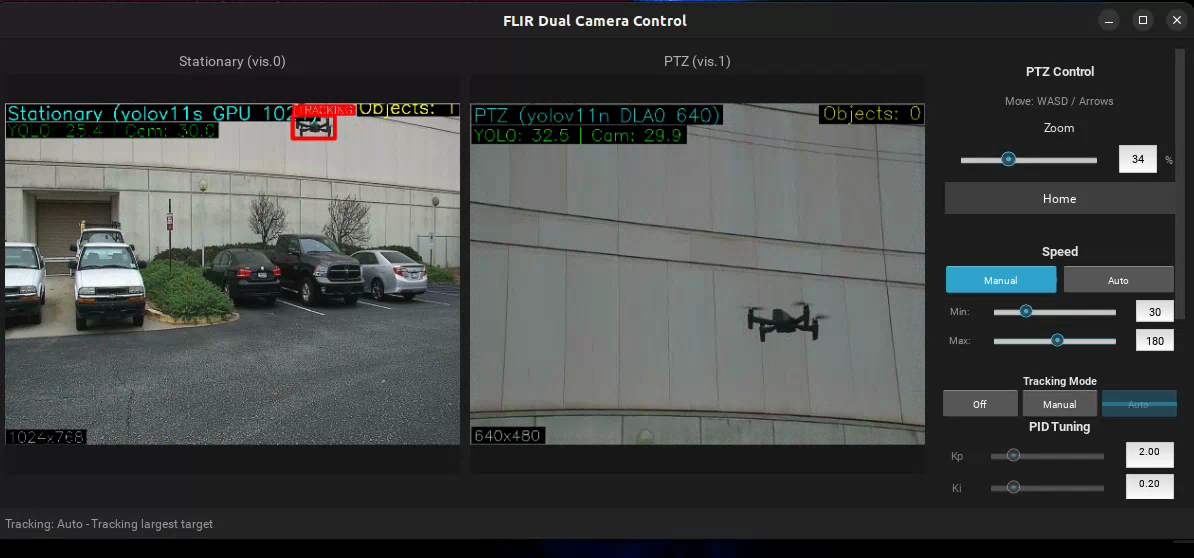
\includegraphics[width=\columnwidth]{figures/fig_drone_tracking.png}
\caption{Active tracking during an outdoor drone test. The stationary camera (left) detects the drone in the wide field and provides bearing cues. The PTZ camera (center) autonomously slews to and tracks the target at optical zoom, maintaining centroid lock via PID control.}
\label{fig:drone_test}
\end{figure}

\begin{figure*}[htbp]
\centering

\includegraphics[width=1.0\textwidth]{figures/fig_tracking_montage.png}
\caption{Temporal montage from the 42-second drone tracking sequence. (a)~System initialization and acquisition phase. (b)~Early tracking with PTZ slewing to target. (c)~Active tracking at medium zoom with drone visible in both cameras. (d)~PTZ detection at higher zoom with green bounding box on target. (e)~Sustained tracking in final flight segment. (f)~End of sequence with maintained lock.}
\label{fig:montage}
\end{figure*}


\subsection{In-Lab Airplane Detection}
In-laboratory testing (Fig.~\ref{fig:inlab}) confirmed that the default YOLOv8n COCO ``airplane'' class detects large, high-resolution aircraft imagery displayed on a monitor but fails on small pixel footprints typical of the wide-angle surveillance view. This motivated training custom detection models on a drone detection dataset and on the Fine-Grained Visual Classification (FGVC) aircraft dataset, which provides ground-up RGB imagery of aircraft at a range of scales and orientations representative of the surveillance scenario.

\begin{figure}[htbp]
\centering
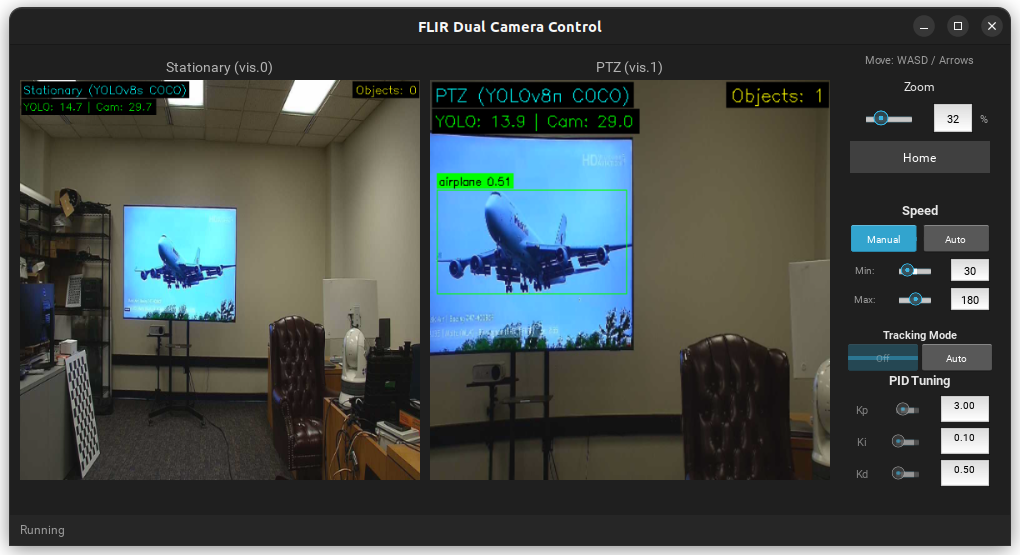
\includegraphics[width=\columnwidth]{figures/fig_inlab_test.png}
\caption{In-laboratory validation. The PTZ camera detects and tracks an aircraft displayed on a monitor using YOLOv8n with COCO weights, confirming the detection pipeline and GUI control interface.}
\label{fig:inlab}
\end{figure}

\subsection{Airplanes Test Case}
For the airplane surveillance application, the primary class is \textit{airplane}. Hard negatives arise from birds, insects near the lens, distant drones, clouds with sharp edges, sensor noise, and specular highlights. The PTZ confirmation step naturally collects informative negatives: wide proposals that are rejected by PTZ as non-airplane are stored as hard negatives with contextual metadata.

Custom YOLO models trained on FGVC aircraft data are intended to replace the COCO-pretrained weights for the wide camera, targeting the small pixel sizes ($<30 \times 30$) that COCO-trained models fail to detect. Benchmarking these custom models against default YOLO classes on a test set containing both long-distance and close-distance aircraft remains ongoing work.

\section{Discussion}

\subsection{Telemetry Synchronization}
Accurate label transfer requires time alignment between wide frames, PTZ frames, and PTZ telemetry. The system logs monotonic timestamps at capture and at inference and records the PTZ telemetry state at the exact time a PTZ frame is captured. If telemetry is sampled asynchronously, interpolation to the frame time reduces geometric error.

\subsection{When PTZ Verification Helps Most}
PTZ verification is most valuable when the wide detector frequently encounters ambiguous, small candidates whose pixel support is insufficient for confident classification. In such regimes, zoom provides additional evidence without changing the wide camera that will ultimately run the detector. This is especially beneficial when the deployment environment differs from training data and when pseudo-labeling alone would be unreliable.

\subsection{Limitations}
The system is constrained by single-PTZ availability and cannot zoom multiple targets simultaneously. Fast-moving targets may leave the PTZ field of view during slew, particularly when latency is high or the wide tracker is unstable. Atmospheric turbulence and haze can reduce the effective benefit of zoom. Direction-only label transfer assumes small parallax; large baselines or nearer targets require depth-aware mapping. The current experimental characterization covers detector throughput and a single drone tracking scenario; larger-scale deployment with multiple target types and varying weather conditions is needed to fully assess operational robustness.

\subsection{Future Work}
The evaluation protocol for full deployment includes three baselines: a wide-only baseline without PTZ confirmation, a PTZ patrol baseline with scripted scanning, and a manual-zoom oracle on an audited subset. Primary metrics include label precision and recall, bounding-box IoU between transferred and audited labels, confidence uplift ($\Delta s = s^p - s^w$), and downstream small-object mAP after training on the constructed dataset. System metrics include slew-to-lock time, dwell time per target, reacquisition success rate, and PTZ availability contention. Ablation studies will isolate contributions from trigger thresholds, motion prediction, zoom scheduling, and label transfer methods. Multi-PTZ configurations can reduce contention and increase throughput via joint scheduling across targets.

\subsection{Safety and Privacy}
The airplane test case naturally focuses on sky regions; nonetheless, deployment constrains PTZ tilt limits and defines privacy-preserving regions to avoid capturing ground-level imagery. These constraints are implemented at the control layer by rejecting commands that enter prohibited zones.

\section{Conclusion}
This paper presented a dual-camera active acquisition system for automated small-object dataset construction. A fixed wide-angle camera with real-time detection provides persistent coverage, while a PTZ camera delivers optical zoom for verification. The system runs on an NVIDIA Jetson Orin AGX, achieving 35.9\,FPS (GPU) and 21.5\,FPS (DLA) through a parallel GPU/DLA inference split that eliminates resource contention. PID-controlled PTZ tracking with MJPEG codec selection minimizes pipeline latency for closed-loop operation. We demonstrated end-to-end functionality through a 42-second outdoor drone tracking test, where the system autonomously acquired and maintained lock on a small aerial target, resolving it from ${\sim}20$ pixels in the wide view to ${\sim}120$ pixels under optical zoom. The active acquisition paradigm provides ground-truth-quality imagery that neither digital zoom nor super-resolution can match, enabling automated dataset construction for small-object regimes where manual annotation is impractical.

\begin{thebibliography}{99}

\bibitem{nikouei2024smallobj}
M. Nikouei et al., ``Small Object Detection: A Comprehensive Survey on Challenges, Techniques, and Real-World Applications,'' \textit{Intelligent Systems with Applications}, vol.\ 25, 2025. doi: \url{https://doi.org/10.1016/j.iswa.2025.200561}

\bibitem{mahaur2022superres}
B. Mahaur, N. Singh, and K. K. Mishra, ``Road object detection: a comparative study of deep learning-based algorithms,'' \textit{Multimedia Tools and Applications}, vol.\ 81, no.\ 10, pp.\ 14247--14282, 2022. doi: \url{https://doi.org/10.1007/s11042-022-12447-5}

\bibitem{rozantsev2017flying}
A. Rozantsev, V. Lepetit, and P. Fua, ``Detecting Flying Objects Using a Single Moving Camera,'' \textit{IEEE Trans.\ Pattern Analysis and Machine Intelligence}, vol.\ 39, no.\ 5, pp.\ 879--892, 2017. doi: \url{https://doi.org/10.1109/TPAMI.2016.2564408}

\bibitem{chen2020survey}
G. Chen, H. Pu, W. Luo, and L. Zhang, ``A Survey of the Four Pillars for Small Object Detection: Multiscale Representation, Contextual Information, Super-Resolution, and Region Proposal,'' \textit{IEEE Trans.\ Systems, Man, and Cybernetics: Systems}, vol.\ 52, no.\ 2, pp.\ 936--953, 2022. doi: \url{https://doi.org/10.1109/TSMC.2020.3005231}

\bibitem{zhang2019zoom}
X. Zhang, Q. Chen, R. Ng, and V. Koltun, ``Zoom to Learn, Learn to Zoom,'' in \textit{Proc.\ IEEE/CVF Conf.\ Computer Vision and Pattern Recognition (CVPR)}, pp.\ 3762--3770, 2019. doi: \url{https://doi.org/10.1109/CVPR.2019.00388}

\bibitem{yolo_flying}
M. Saavedra-Ruiz, A. Morin, and L. Bhatt, ``Real-Time Flying Object Detection with YOLOv8,'' \textit{arXiv preprint arXiv:2305.09972}, 2023. doi: \url{https://doi.org/10.48550/arXiv.2305.09972}

\bibitem{ptz_eval}
E. Borreglero, M. Lucena, J. Fuertes, and N. Perez de la Blanca, ``Evaluation of Trackers for Pan-Tilt-Zoom Scenarios,'' \textit{arXiv preprint arXiv:1711.04260}, 2017. doi: \url{https://doi.org/10.48550/arXiv.1711.04260}

\bibitem{ptz_reproducible}
P. Carr and R. Hartley, ``Reproducible Evaluation of Pan-Tilt-Zoom Tracking,'' in \textit{Proc.\ IEEE Int.\ Conf.\ Image Processing (ICIP)}, 2015. doi: \url{https://doi.org/10.1109/ICIP.2015.7351162}

\bibitem{active_ptz}
J. Feng, Y. Shi, and Z. Wang, ``Active Visual Perception Enhancement Method Based on Deep Reinforcement Learning,'' \textit{Electronics}, vol.\ 13, no.\ 9, p.\ 1654, 2024. doi: \url{https://doi.org/10.3390/electronics13091654}

\bibitem{anomalous_ptz}
G. Suarez-Fernandez, J. Garcia, and F. Lecumberry, ``Anomalous object detection by active search with PTZ cameras,'' \textit{Expert Systems with Applications}, vol.\ 184, p.\ 115150, 2021. doi: \url{https://doi.org/10.1016/j.eswa.2021.115150}

\bibitem{vigia_ptz}
A. Pedrosa, T. Marques, and J. Nascimento, ``VIGIA-E: Density-Aware Patch Selection for Efficient Video Surveillance with PTZ Cameras,'' in \textit{Proc.\ 25th Int.\ Conf.\ Computer Analysis of Images and Patterns (CAIP)}, 2025. doi: \url{https://doi.org/10.1007/978-3-032-04968-1_23}

\bibitem{self_training}
S. Li, M. Tian, and L. Chen, ``Adaptive Self-Training for Object Detection,'' in \textit{Proc.\ IEEE/CVF Int.\ Conf.\ Computer Vision Workshops (ICCVW)}, 2023. doi: \url{https://doi.org/10.1109/ICCVW60793.2023.00102}

\bibitem{self_training_enh}
H. Park, J. Lee, and S. Kim, ``Improving Object Detection Accuracy with Self-Training Based on Bi-Directional Pseudo Label Recovery,'' \textit{Electronics}, vol.\ 13, no.\ 12, p.\ 2230, 2024. doi: \url{https://doi.org/10.3390/electronics13122230}

\bibitem{active_learning_survey}
A. Morales-Hernandez, I. Kabir, and M. Arif, ``Ten Years of Active Learning Techniques and Object Detection: A Comprehensive Survey,'' \textit{Applied Sciences}, vol.\ 13, no.\ 10, p.\ 6181, 2023. doi: \url{https://doi.org/10.3390/app13169110}

\bibitem{active_learning_ppod}
C. Wu, P. Sun, and R. Zhu, ``Plug and Play Active Learning for Object Detection,'' in \textit{Proc.\ IEEE/CVF Conf.\ Computer Vision and Pattern Recognition (CVPR)}, 2024. doi: \url{https://doi.org/10.1109/CVPR52733.2024.01684}

\bibitem{ptz_latency_pelco}
Pelco, ``What is the Measured Latency on Esprit Compact PTZ Cameras?,'' Pelco Support Article, 2024. [Online]. Available: \url{https://support.pelco.com/s/article/What-is-the-Measured-Latency-on-Esprit-Compact-PTZ-Cameras}

\bibitem{ptz_latency_optics}
PTZOptics, ``Fixing IP-Based Latency \& Sync Issues on PTZOptics Cameras,'' PTZOptics Knowledge Base, 2024. [Online]. Available: \url{https://community.ptzoptics.com/s/article/Fixing-IP-Based-Latency-Sync-Issues-on-PTZOptics-Cameras}

\bibitem{nvidia_jetson_benchmarks}
NVIDIA, ``NVIDIA Jetson AI Lab Benchmarks,'' NVIDIA Jetson AI Lab, 2024. [Online]. Available: \url{https://www.jetson-ai-lab.com/benchmarks.html}

\end{thebibliography}

\end{document}
